% A simple Pentagon with TiKZ
% Author: Christoph Gerum <gerum@informatik.uni-tuebingen.de>
\documentclass{standalone}

\usepackage{tikz}

\begin{document}

%circle
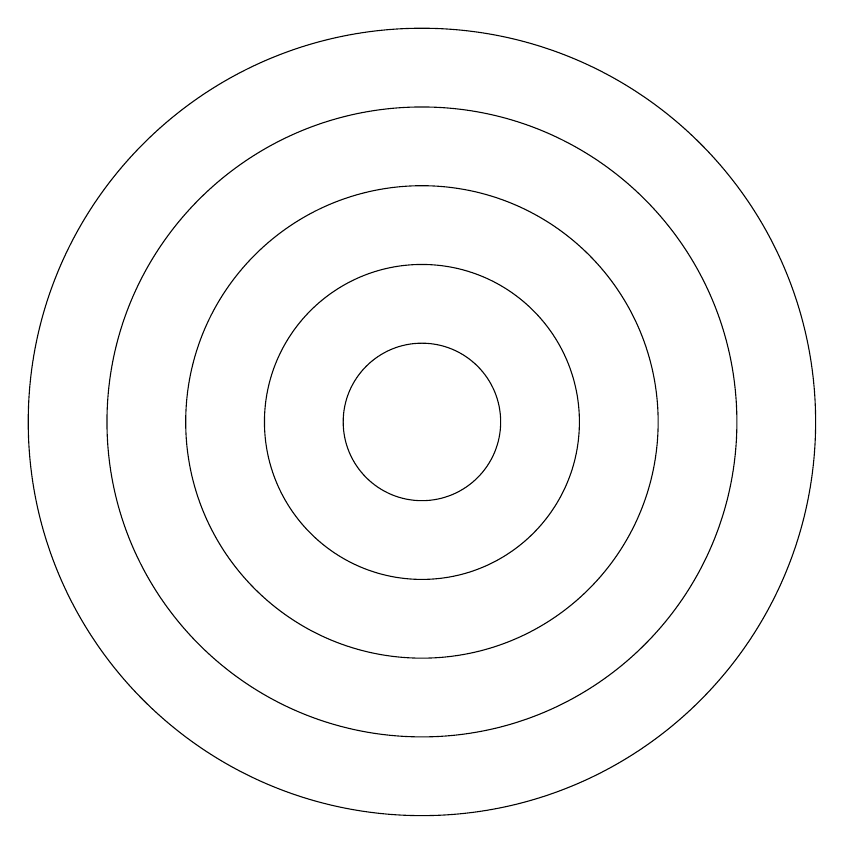
\begin{tikzpicture}
%  \draw [step=0.25cm,color=gray] (-1, -1) grid (1, 1);
  
  \path (0,0) coordinate (origin);

  \draw (origin) circle (1cm);
  \draw (origin) circle (2cm);
  \draw (origin) circle (3cm);
  \draw (origin) circle (4cm);
  \draw (origin) circle (5cm);

\end{tikzpicture}

%arc

\begin{tikzpicture}
  \draw (0:1cm) -- (0:4cm) 
        arc(0:60:4cm) -- (60:1cm) arc(60:0:1cm) -- cycle;
\end{tikzpicture}


\end{document}
